\documentclass[conference]{IEEEtran}
\IEEEoverridecommandlockouts
\usepackage{cite}
\usepackage{amsmath,amssymb,amsfonts}
\usepackage{booktabs}
\usepackage{algorithmic}
\usepackage{graphicx}
\usepackage{textcomp}
\usepackage{xcolor}
\usepackage{float}     
\usepackage{placeins}
\usepackage{tikz}
\usetikzlibrary{shapes.geometric}
\def\BibTeX{{\rm B\kern-.05em{\sc i\kern-.025emb}\kern-.08em
    T\kern-.1667em\lower.7ex\hbox{E}\kern-.125emX}}
\begin{document}

\title{Implementação de filtros FIR para redução do espalhamento espectral causado pela saturação do sinal em Dual-Band}

\author{\IEEEauthorblockN{Clayson G. S. de Oliveira and Luis Schuartz}
\IEEEauthorblockA{Group of Integrated Circuits and Systems (GICS) – Departamento de Engenharia elétrica} Federal Universidade do Paraná, Curitiba, Brasil\\ gabrielclayson@gmail.com}

\maketitle

\begin{abstract}
Resumo aqui.
\end{abstract}

\begin{IEEEkeywords}
Filtro FIR, Banda dupla concorrente, Amplificador de Potência, Predistorsor digital, Saturação do DPD, Coeficientes.
\end{IEEEkeywords}

\section{Introdução}


Com o passar dos anos, a transmissão de sinais passou a ocupar um papel cada vez mais relevante no cotidiano. Consequentemente, a tecnologia envolvida nesse processo evoluiu significativamente, exigindo maior refinamento, linearidade e eficiência. Dentro desse contexto, o amplificador de potência (PA) recebe atenção crítica, por ser um componente essencial situado antes da antena transmissora e responsável pela amplificação do sinal antes da transmissão. Para que o equipamento seja eficiente, é necessário que opere próximo ao seu limiar de saturação, sem ultrapassá-lo, a fim de evitar distorções no sinal.

Entretanto, o próprio processo de amplificação pode introduzir distorções, comprometendo a integridade da informação transmitida. Para mitigar esse efeito, emprega-se o pré-distorsor digital (DPD), implementado de forma a gerar uma distorção inversa à provocada pelo PA. Assim, quando o amplificador atua sobre um sinal previamente distorcido de maneira inversa, o resultado é uma saída linearizada.

O processo de saturação do sinal ocorre antes da aplicação do pré-distorsor, com o objetivo de elevar sua potência média. Essa etapa consiste em realizar um corte (\textit{hard clipping}) na envoltória equivalente, limitando a tensão a um determinado limiar $L$. Tal procedimento busca controlar o comportamento do sinal, uma vez que a limitação natural imposta pelo PA seria caótica e imprevisível. Após o corte, o sinal é separado, e o trecho saturado é reintroduzido, já que, tratando-se de uma comunicação em banda dupla, qualquer modificação na envoltória influencia ambas as informações.

Embora a saturação aumente a potência média do sinal, ela também provoca espalhamento espectral, podendo ultrapassar os limites estabelecidos por órgãos reguladores. Diante disso, o presente trabalho tem como objetivo implementar um filtro FIR capaz de reduzir o espalhamento espectral causado pela saturação, preservando a fase do sinal e evitando distorções adicionais, além de aplicar técnicas que minimizem a ordem do filtro, visando uma implementação prática e eficiente.


\section{DPD saturation and FIR filters}

In the equivalent envelope representation, which is crucial for the transmission of signals in a concurrent dual-band scenario, both signals modulated at different frequencies are represented in the same model. The equivalent envelope \cite{b2} for a concurrent dual-band system is given by

\begin{equation}
    x(n)=x_1(n) e^{\frac{-j\Delta \omega \left(n-1\right)}{f_s}}+x_2(n)e^{\frac{j\Delta \omega \left(n-1\right)}{f_s}},
    \label{eq1}
\end{equation}

\noindent where $x_1(n)$ is the signal from channel 1, $x_2(n)$ is the signal from channel 2, $f_s$ is the sampling frequency, and $\Delta \omega$ is the difference between the carriers of the transmitted signals calculated by

\begin{equation}
    \Delta\omega = \dfrac{\omega_2 - \omega_1}{2}.
\end{equation}
    
\subsection{Saturation for dual-band transmission}

In order to obtain better efficiency, before sending the signal to the linearized system, the signal can be clipped. Clipping the signal reduces the difference between the maximum and average amplitude, which allows the PA to reach higher efficiency. The saturated signal, $x_c(n)$ at a threshold $L$ is \cite{b2}

\begin{equation}
x_c(n) = 
\begin{cases} 
x(n), & \text{if } |x(n)| \leq L \\
L \exp(j \angle x(n)), & \text{if } |x(n)| > L 
\end{cases}.
\label{eq:clip}
\end{equation}

Considering only one signal band, (\ref{eq:clip}) is already satisfactory because the equivalent envelope corresponds to its own channel. However, for a dual-band signal, $x_1$ and $x_2$ partly assume the outside $|x(n)| - L$. Thus, $x_c(n)$ is made by $x_{1c}$ and $x_{2c}$. Two approaches are known to calculate $x_{1c}$ and $x_{2c}$, the sum and division methods. The sum approach shows better results \cite{b3}, thus this work is limited to the sum approach.

\subsection{Sum method}

In sum method absolute surplus of equivalent envelope are assigned to the channels, while maintaining the original phase. Having $z(n) = |x(n)| - L$, the saturated envelope of each channels 1 and 2 can be expressed by \cite{b2} 

\begin{equation}
    x_{1c}(n) =
\begin{cases} 
    x_1(n), & \text{if } |x(n)| \leq L \\ 
    \left(\frac{|x_i(n)| - z(n)}{2}\right) e^{j\angle x_1(n)}, & \text{if } |x(n)| > L
\end{cases}.
\label{eq3}
\end{equation}

\noindent and

\begin{equation}
    x_{2c}(n) =
\begin{cases} 
    x_2(n), & \text{if } |x(n)| \leq L \\ 
    \left(\frac{|x_2(n)| - z(n)}{2}\right) e^{j\angle x_2(n)}, & \text{if } |x(n)| > L
\end{cases},
\label{eq4}
\end{equation}

\noindent respectively. Once each channel receives saturation, the traditional DPD for dual-band is used.

\subsection{Filter and windowing}

The simplest method for designing an FIR filter is called the windowing method, applying a window with the desired response in frequency. To an ideal impulse response $h_d(n)$, the frequency response can be represented by \cite{b4}

\begin{equation}
    H_d(e^{j\omega}) = \sum_{n=-\infty}^{\infty} h_d(n) e^{-j\omega n}.
\end{equation}

Once $H_d(e^{j\omega})$ is the impulse response sequence in the frequency, the impulse response in the time-domain is

\begin{equation}
    h_d(n) = \frac{1}{2\pi} \int_{-\pi}^{\pi} H_d(e^{j\omega}) e^{j\omega n} \, d\omega.
\end{equation}

A simple way to obtain the filter from $h_d(n)$ is to truncate it, that is, define a system with impulse response given by

\begin{equation}
    h[n] = \begin{cases}
        h_d[n], & 0\leq n \leq M \\
        0, & \textrm{otherwise}
    \end{cases},
\end{equation}

\noindent where $h(n)$ it is typically represented as a product of the impulse response and a window of finite duration $w(n)$.

Windowing is part of the digitalization technique used to limit the spectral response. However, different types of windowing, such as Hanning, Hamming, and Kaiser, also contribute with their properties in the frequency domain, and consequently, can demonstrate better performance in the desired application.

\section{Proposed Filtered 2D DPD saturation}

As presented in Section II, DPD saturation for the concurrent dual-band scenario occurs for each channel once the equivalent envelope is known. Saturation increases efficiency at the cost of spectral growth near each channel separately. However, the current saturation technique also causes floor spectrum growth. Therefore, the filter is implemented individually for each channel, configured to reduce the floor spectrum growth while still allowing spectral growth near the desired channel.

Figure~\ref{fig1} illustrates the implementation scheme of the proposed approach, which integrates an FIR filter into the overall response of the system. Considering this overview, it is clear that the use of IIR (Infinite Impulse Response) filters would not be suitable for our project, because we need a system with linear phase, which IIR filters do not guarantee, and ultimately it can distort our signal \cite{b4}. The system represents only the digital implementation of saturation, filtering and predistortion. The block Env represents the equivalent envelope detector (\ref{eq1}), the block Sat denotes the saturation block as defined by (\ref{eq3}) and (\ref{eq4}), and Fil refers to the filtering block. Here, $x_{1c}$ and $x_{2c}$ represent the saturated signals, as defined by (\ref{eq3}) and (\ref{eq4}), respectively. Similarly, $x_{1f}$ and $x_{2f}$ denote the filtered signals for channels 1 and 2, respectively, while $x_{1f}'$ and $x_{2f}'$ correspond to the predistorted signals for each channel.

\begin{figure}[htpb!]
\centering

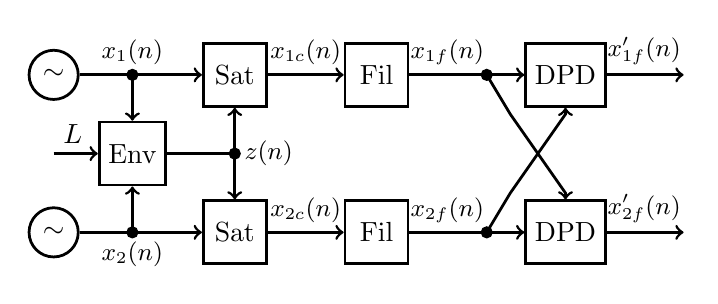
\begin{tikzpicture}[scale = 1]
\node[draw,line width = 1pt,minimum size = 0.5cm,circle] at(-3,1) (in1) {$\sim$};
\node[draw,line width = 1pt,minimum size = 0.5cm,circle] at(-3,-1) (in2) {$\sim$};


\node[draw,line width = 1pt,minimum size = 0.8cm] at(-2,0) (z) {Env};


\node[draw,line width = 1pt,minimum size = 0.8cm] at(-0.7,1) (sat1) {Sat};
\node[draw,line width = 1pt,minimum size = 0.8cm] at(-0.7,-1) (sat2) {Sat};

\node[draw,line width = 1pt,minimum size = 0.8cm] at(1.1,1) (F1) {Fil};
\node[draw,line width = 1pt,minimum size = 0.8cm] at(1.1,-1) (F2) {Fil};


\node[draw,line width = 1pt,minimum size = 0.8cm] at(3.5,1) (dpd1) {DPD};
\node[draw,line width = 1pt,minimum size = 0.8cm] at(3.5,-1) (dpd2) {DPD};


\draw [->,line width = 1pt] (-3,0) -- (z.west);


\draw [->,line width = 1pt] (in1.east) -- (-2,1) -- (z.north);
\draw [->,line width = 1pt] (in2.east) -- (-2,-1) -- (z.south);


\draw [->,line width = 1pt] (z.east) -- (-0.7,0) -- (sat1.south);
\draw [->,line width = 1pt] (-0.7,0) -- (sat2.north);


\draw [->,line width = 1pt] (-2,1) -- (sat1.west);
\draw [->,line width = 1pt] (-2,-1) -- (sat2.west);


\draw [->,line width = 1pt] (sat1.east) -- (F1.west);
\draw [->,line width = 1pt] (sat2.east) -- (F2.west);

\draw [->,line width = 1pt] (F1.east) -- (dpd1.west);
\draw [->,line width = 1pt] (F2.east) -- (dpd2.west);


\draw [->,line width = 1pt] (2.5,1) -- (2.8,0.5) -- (3.5,-0.5) -- (dpd2.north);
\draw [->,line width = 1pt] (2.5,-1) -- (2.8,-0.5) -- (3.5,0.5) -- (dpd1.south);


\draw [->,line width = 1pt] (dpd1.east) -- (5,1);
\draw [->,line width = 1pt] (dpd2.east) -- (5,-1);


\filldraw [black] (-2,1) circle (2pt);
\filldraw [black] (-2,-1) circle (2pt);
\filldraw [black] (-0.7,0) circle (2pt);
\filldraw [black] (2.5,1) circle (2pt);
\filldraw [black] (2.5,-1) circle (2pt);


\node[above right]at(-3,0){$L$};


\node[above]at(-2,1){\small $x_1(n)$};
\node[below]at(-2,-1){\small $x_2(n)$};
\node[right]at(-0.7,0){\small $z(n)$};


\node[above]at(0.2,1){\small $x_{1c}(n)$};
\node[above]at(0.2,-1){\small $x_{2c}(n)$};

\node[above]at(2,1){\small $x_{1f}(n)$};
\node[above]at(2,-1){\small $x_{2f}(n)$};


\node[above]at(4.5,1){\small $x'_{1f}(n)$};
\node[above]at(4.5,-1){\small $x'_{2f}(n)$};
\end{tikzpicture}
\caption{Proposed system with filters for concurrent dual-band DPD saturation.}
\label{fig1}
\end{figure}

The filters are designed in the frequency domain using the saturated signal band-width, which is defined to ensure that DPD saturation maintains signal amplitude compression while minimizing the spectral floor growth. In practice, a double signal band-width is selected as filter cut-off.

The filter is synthesized in Python by \textit{firwin} from \textit{scipy.signal} library. The function returns the filter impulse response specified by the number of coefficients ($C = M+1$), where $M$ is the filtering order; the normalized frequency $2f_c/f_s$, where $f_c$ is the selected cut-off frequency and $f_s$ is the sample frequency; and the desired windowing method. The signals are filtered in time-domain by convolution operation.

\section{Validation tests}

\subsection{Tests setup}

The tests were performed with Python, Octave and Cadence Virtuoso software. Python was used for data processing, specifically for data treatment, saturation, windowing, and filtering. For integration into Python, well-known libraries for data processing were utilized, including \textit{pandas}, \textit{sciPy}, \textit{numPy}, and other integrated tools. Octave was used to evaluate the power spectral density (PSD) using the fast Fourier transform (FFT) and to generate plots.

Modulation data were obtained from Cadence Virtuoso as follows: Channel 1 was modulated using the IEEE 802.11n standard, while channel 2 used the LTE standard. Both signals had a bandwidth of 20~MHz and a sampling rate of 120~MHz. Cadence Virtuoso was also used to evaluate the error vector magnitude (EVM). The standard limits for PSD were obtained from Cadence Virtuoso. Data were transferred between Cadence Virtuoso and Python using text files. To obtain the signals, visualize the constellation and calculate the EVM, envelope simulations were performed in Cadence Virtuoso.

Filters are designed to have double bandwidth cut-off frequencies. Additionally, the order $M$ is set to 50 and 80 for channels 1 and 2, respectively. The filter orders were chosen to minimize in-band ripple.

\subsection{Obtained results}

Figure \ref{fig2} shows the equivalent envelope (\ref{eq1}) for the original $x_1$ and $x_2$, as well as after the saturation procedure using the sum method, i.e., with $x_{1c}$ and $x_{2c}$. In fact, the equivalent envelope exhibits significant amplitude compression after the saturation procedure, allowing the linearized circuit to achieve high efficiency without model extrapolation. The selected threshold $L$ will be discussed alongside the PSD results.

\begin{figure}[htpb!]
\centering
\centerline{\includegraphics[width=1\linewidth, trim = 0.5cm 0cm 1.5cm 1cm, clip]{sinal_saturado.pdf}}
\caption{Equivalent envelope for a concurrent dual-band system without and with saturation.}
\label{fig2}
\end{figure}

Figures \ref{fig3} and \ref{fig4} show the filtering results after the saturation block for Channels 1 and 2, respectively. Each figure also includes the unfiltered signals from the saturation block and the respective standard mask. In both figures, only the sum method was used with a threshold of $L=44$\% of equivalent envelope amplitude. The selected threshold voltage was chosen to achieve the maximum PSD with filters while respecting the standard mask; in other words, it represents the best-case scenario achievable with the filtering block implementation. Other threshold voltages are suppressed to obtain a clean image.

\begin{figure}[htpb!]
\centering
\centerline{\includegraphics[width=1\linewidth, trim = 4.0cm 8.5cm 3.5cm 9cm, clip]{wifi_filtros.pdf}}
\caption{PSD of channel 1, comparing saturation with and without filtering for different windowing techniques.}
\label{fig3}
\end{figure}

\begin{figure}[htpb!]
\centering
\centerline{\includegraphics[width=1\linewidth, trim = 4.0cm 8.5cm 3.5cm 9cm, clip]{LTE_filtros.pdf}}
\caption{PSD of channel 2, comparing saturation with and without filtering for different windowing techniques.}
\label{fig4}
\end{figure}

Analyzing the results in figs. \ref{fig3} and \ref{fig4}, it is noticeable that using only saturation with the selected threshold causes the noise floor to increase, thereby rendering the application unviable. However, by applying filters, regardless of the windowing technique used, the system is able to meet the regulations. Among the windowing techniques, the Hamming window was the most selective, effectively reducing undesired power, and was therefore chosen for the subsequent results.

The main uncertainty regarding the previous PSD results is how they change the signals in time-domain. It was expected that each signal remained uncompromised while the equivalent envelope stayed saturated. 

Figures \ref{fig5} and \ref{fig6} show the results for channels 1 and 2 over time, respectively. The signals after filtering exhibit a decrease in amplitude, which can also reduce the peak-to-average power ratio (PAPR) of each channel. However, the signals maintain the same original shape. 

\begin{figure}[htpb!]
\centering
\centerline{\includegraphics[width=1\linewidth, trim = 4.0cm 8.5cm 4.5cm 9cm, clip]{Wifi_tempo.pdf}}
\caption{Amplitude of channel 1 with saturation and filtering.}
\label{fig5}
\end{figure}

\begin{figure}[htpb!]
\centering
\centerline{\includegraphics[width=1\linewidth, trim = 4.0cm 8.5cm 4.5cm 9cm, clip]{LTE_tempo.pdf}}
\caption{Amplitude of channel 2 with saturation and filtering.}
\label{fig6}
\end{figure}

In addition to each channel in the time-domain, the amplitude of the equivalent envelope for filtered signals must remain below the threshold. Figure \ref{fig7} shows the equivalent envelope of the original signal, as well as the saturated and filtered signals. As illustrated in the figure, the filter does not raise the equivalent envelope above the limit.

\begin{figure}[htpb!]
\centering
\centerline{\includegraphics[width=1\linewidth, trim = 0.5cm 0cm 1.5cm 1cm, clip]{sinal_saturado_filtrado.pdf}}
\caption{Equivalent envelope for a concurrent dual-band system of proposed system.}
\label{fig7}
\end{figure}

After performing the PSD and time-domain amplitude tests, EVM tests must be conducted to confirm in-band signal quality by comparing the filtered and unfiltered signals. Table~\ref{tab1} presents the EVM results for the signals after saturation and after filtering. A negligible difference is observed in the EVM degradation. Specifically, only channel 1 experiences a loss of 0.2 percentage points, indicating that the inclusion of the filter did not cause any degradation of the in-band information.

\begin{table}[htpb!]
    \centering
    \caption{EVM results of saturated and filtered signals for channels 1 and 2.}
    \begin{tabular}{cccc}
        \toprule
        & \textbf{With filter} & \textbf{Without filter} \\
        \midrule
        \textbf{Channel 1} & 7.1\% & 7.3\% \\
        \textbf{Channel 2} & 8.0\% & 8.0\% \\
        \bottomrule
    \end{tabular}
    \label{tab1}
\end{table}

Table \ref{tab2} summarizes the PAPR measurements for channels 1 and 2, as well as the equivalent envelope (Eq. envelope). On the one hand, the PAPR of unsaturated and saturated signals for channels 1 and 2 remains practically the same. They change slightly, which can be justified since the average power of each channel has already changed. A similar interpretation applies to the filtered signals. On the other hand, the equivalent envelope undergoes a more significant change. While the saturated envelope imposes a hard limit on the PAPR, reducing it by about 4 dB compared to the unsaturated signal, the filter partially restores the PAPR, increasing it by approximately 0.6~dB. Nevertheless, this undesired PAPR increase is justified, as the filtering allows for a considerable threshold reduction.

\begin{table}[htpb!]
    \centering
    \caption{PAPR results of unsaturated, saturated and filtered signals of channels 1, 2 and the equivalent envelope.}
   \begin{tabular}{c|ccc} \toprule
 & \textbf{\begin{tabular}[c]{@{}c@{}}PAPR\\ Channel 1\end{tabular}} & \textbf{\begin{tabular}[c]{@{}c@{}}PAPR\\ Channel 2\end{tabular}} & \textbf{\begin{tabular}[c]{@{}c@{}}PAPR\\ Eq. envelope\end{tabular}} \\ \midrule
\textbf{Unsaturated} & 8.43 dB & 8.24 dB & 9.09 dB \\
\textbf{Saturated} & 8.89 dB & 8.03 dB & 5.28 dB \\
\textbf{Filtered} & 8.35 dB & 7.27 dB & 5.9 dB \\  \bottomrule
\end{tabular}
    \label{tab2}
\end{table}

\section{Conclusions}

The literature shows that the use of saturation for concurrent dual-band systems allows the PA, linearized by DPD, to achieve high efficiency. However, the spectral growth of each channel can easily exceed the standard limits, which limits the applicability of the technique. Thus, this work evaluates the inclusion of filtering to limit spectral growth. The results of the proposed integration demonstrate that filtering effectively limits the spectral growth without significant in-band degradation compared to the DPD saturation technique in the literature. Specifically, the EVM loss is below 0.5 percentage points, and the PAPR of the equivalent envelope increased by 0.6~dB after the implemented filtering.


\begin{thebibliography}{00}
\bibitem{b1} L. Schuartz, R. G. Silva, A. T. Hara, A. A. Mariano, B. Leite, and E. G. Lima, ``Concurrent Tri-band CMOS Power Amplifier Linearized by 3D Improved Memory Polynomial Digital Predistorter,'' Circuits Syst Signal Process, vol. 40, pp. 2176–2208, 2021.
\bibitem{b1_2} T. Kobal, Y. Li, X. Wang, and A. Zhu, ``Digital Predistortion of RF Power Amplifiers With Phase-Gated Recurrent Neural Networks,'' in IEEE Transactions on Microwave Theory and Techniques, vol. 70, no. 6, pp. 3291-3299, June 2022.
\bibitem{b1_3} S. Wang, W. Cao, R. Hou and T. Eriksson, ``A Digital Predistortion for Concurrent Dual-Band Power Amplifier Linearization Based on Periodically Nonuniform Sampling Theory,'' in IEEE Transactions on Microwave Theory and Techniques, vol. 70, no. 1, pp. 466-475, Jan. 2022.
\bibitem{b1_4} B.E. Shinde, and V. Vijayabaskar, ``An Opportunistic Coexistence Analysis of LTE and Wi-Fi in Unlicensed 5 GHz Frequency Band,'' Wireless Pers Commun, vol 130, 269–280, 2023.
\bibitem{b1_5} G. Naik, J. Liu, and J. M. J. Park, ``Coexistence of Wireless Technologies in the 5 GHz Bands: A Survey of Existing Solutions and a Roadmap for Future Research,'' in IEEE Communications Surveys \& Tutorials, vol. 20, no. 3, pp. 1777-1798, 2018. 
\bibitem{b1_6} L. Schuartz, E. L. Santos, B. Leite, A. A. Mariano, and E. G. Lima, ``Traditional and Saturated Digital Baseband Predistorters for Wireless Transmitters,'' Proceedings of the 33rd South Symposium on Microelectronics, Curitiba, 2018.
\bibitem{b2} L. Schuartz, and E. G. Lima, ``Saturation Approach for Dual-Band Transmission with Pre-Distortion for PA Efficiency Increase,'' Brazilian Archives of Biology AND Technology, vol. 67, p. 1-9, 2024.
\bibitem{b3} L. O. L. Miliavacca, and L. Schuartz, ``Análise dos efeitos da saturação do DPD de banda dupla concorrente,'' Procedings of Siminários de Microeletrônica do Paraná, vol. 7, 2024. 
\bibitem{b4} A. V. Oppenheim, and R. W. Schafer, Processamento em tempo discreto de sinais. 3rd ed. São Paulo: Pearson, 2013.
\bibitem{b5}IEEE 802.11n-2009, ``IEEE Standard for Information technology,'' in IEEE Std 802.11p-2010, pp.1-51, July 2010.

\end{thebibliography}
\end{document}
